\chapter{Klassische Mechanik}

\section{Abriss der Newtonschen Mechanik}

Problemstellung der klassischen Mechanik: Orte $\vec{r}_i$ und Geschwindigkeiten $\vec{v}_i$ zur Zeit $t$ gegeben für ein System von Massenpunkten mit $1 \le i \le N$ (also $N$ Massenpunkte).

Es wirken äußere Kräfte $\vec{F}$ und Kräfte zwischen den Teilchen $i$ und $j$ ($i \neq j$): $\vec{F}_{ij}$.

Wie lauten die \textbf{kinematischen Größen} $\vec{r}_i(t)$ und $\vec{v}_i(t) = \dvec{r}_i(t)$ (wobei $\dvec{r} = \sdiv{\vec{r}}{t}$) für beliebige Zeiten $t$ danach?

Die kinematischen Größen $\vec{r}_i(t)$ (und $\dvec{r}_i(t)$) werden als Lösungen gewöhnlicher Differentialgleichungen gefunden; das sind die \textbf{Bewegungsgleichungen}.

Neben diesen kinematischen Größen gibt es die wichtigen Begriffe \textbf{Kraft}, \textbf{Masse}, \textbf{Impuls} und \textbf{Energie}.


\textbf{Kraft} vektorielle Größe, meistens $\vec{F}$ (manchmal auch $\vec{K}$); ist immer die Ursache von Bewegung oder der Änderung von Bewegungszuständen $\rightarrow$ kräftefrei $\rightarrow$ Bewegung unverändert 
	
Das führt auf die \textbf{Newtonschen Gesetze}: 
\begin{description}
	\item[lex prima (Galileisches Trägheitsgesetz)] es gibt Initialsysteme, in denen ein kräftefreier Körper (= Massepunkt) ruht oder sich gradlinig gleichförmig bewegt
		
	\textbf{Definition}: Jeder Massepunkt setzt der Einwirkung von Kräften einen \textbf{Trägheitswiderstand} entgegen = Masse, oder besser: \textbf{träge Masse} (Formelzeichen: $m$)
		
	\textbf{Definition}: \textbf{Impuls} $\vec{p} = m \vec{v}$
		
	\item[lex secunda (Bewegungsgesetz)] $\dvec{p} = \vec{F}$; meistens ist $m$ unveränderlich, dann ist $\dvec{v} = \sdiv{}{t} \vec{v} = \vec{a}$ und $\vec{F} = m \vec{a}$.
		
	\item[lex tertia (actio = reactio)] $\vec{F}_{ij} = - \vec{F}_{ji}$ 
	
	\begin{figure}
		\centering
		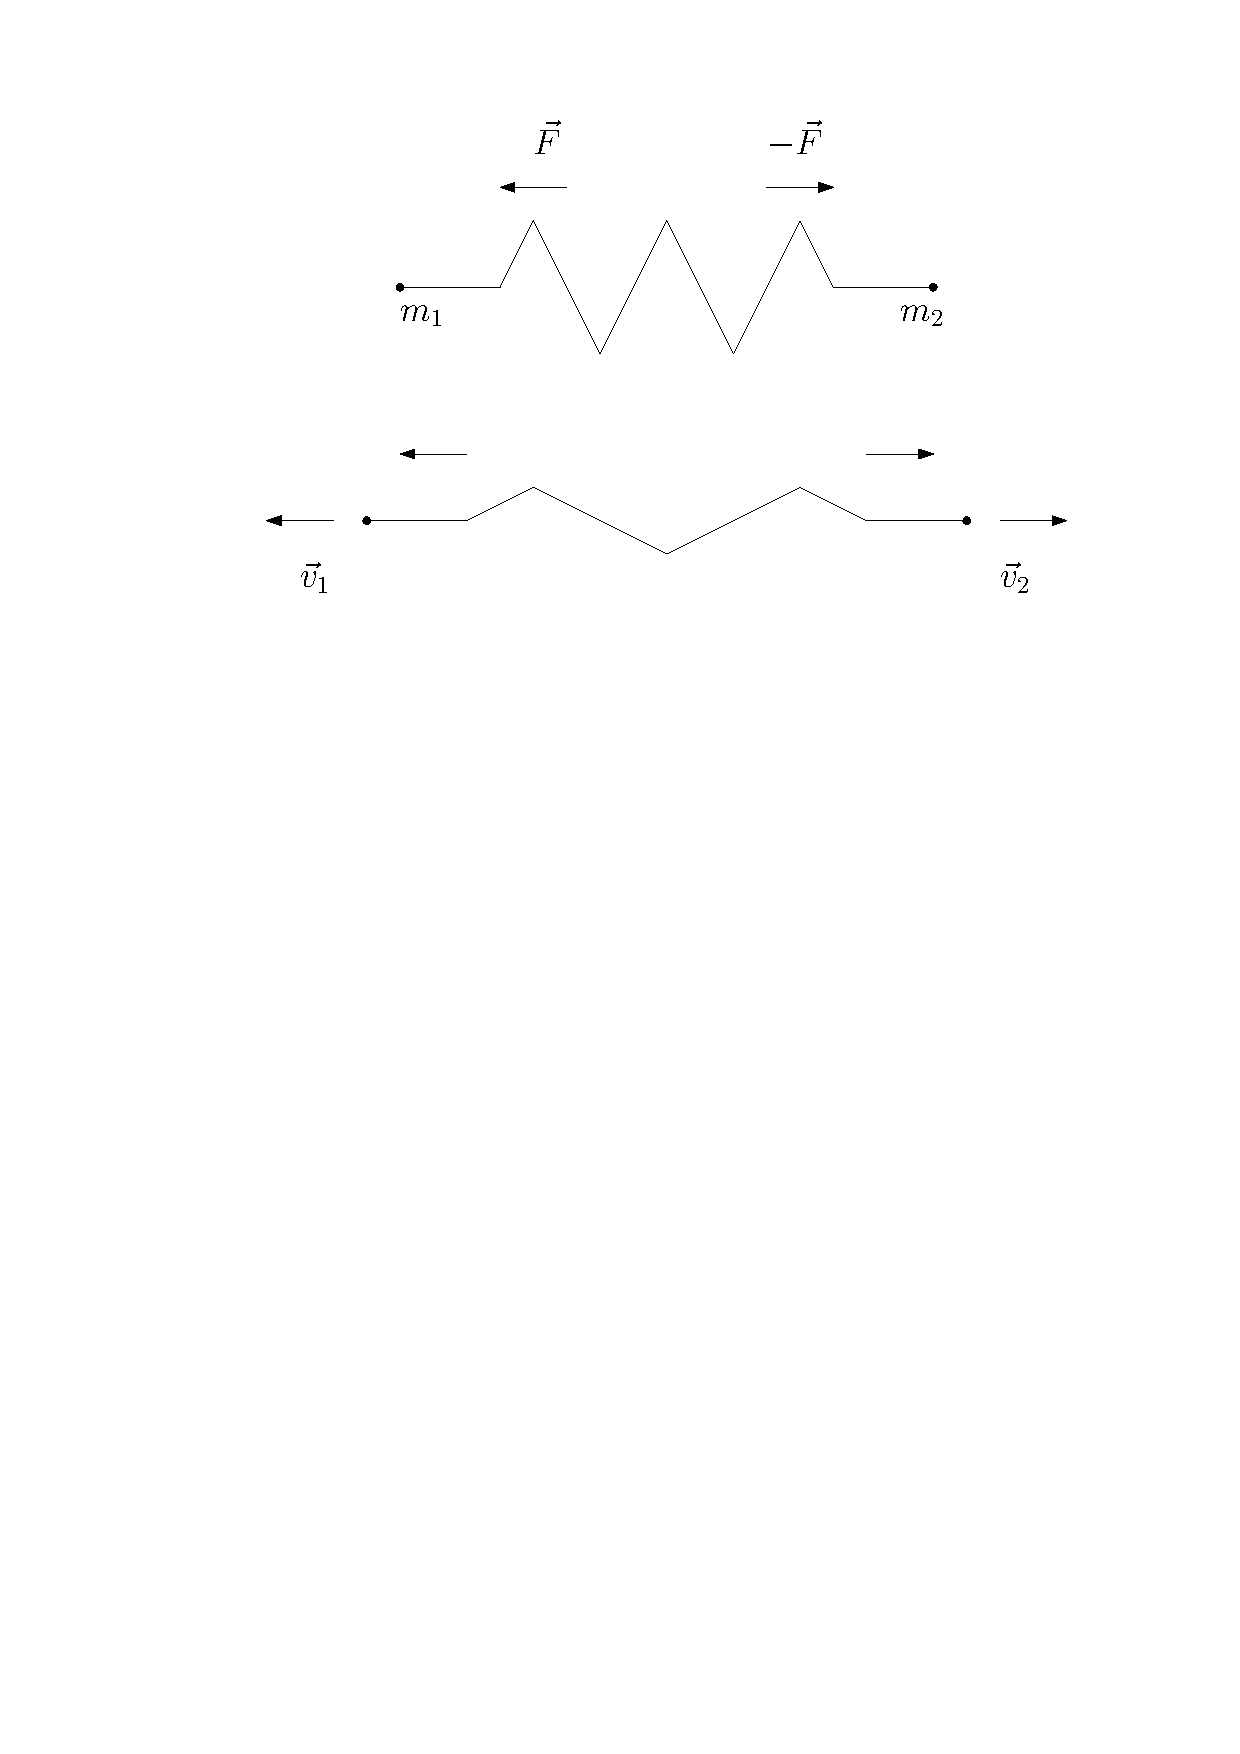
\includegraphics[scale=0.5]{figures/ch1/feder}
		\caption{actio = reactio bei einer Feder}
		\label{fig:ch1_feder}
	\end{figure}

	
	Beobachtung aus Abbildung \ref{fig:ch1_feder}: $\frac{v_1}{v_2} = \frac{m_2}{m_1}$, unabhängig von $\vec{F}$; das führt auf die Massendefinition
\end{description}

Wichtige Beispiele für Kräfte:

\begin{itemize}
	\item Gravitationskraft (schwere Masse = träge Masse): $\vec{F} = -\gamma \frac{M m}{r^2} \hat{r}$, wobei $\hat{r} = \frac{\vec{r}}{\mabs{\vec{r}}}$ und $\gamma$ die Gravitationskonstante ist
	
		Skizze
	
		Speziell auf der Erde: $r = r_e$, $M = M_e$, $\gamma$
		
		Damit $F = \underbrace{\gamma \frac{M_e}{r_e^2}}_{=: g} m = mg$ und $g \approx 9.81 m s^{-2}$; die Kraft zeigt nach unten, deswegen nur noch $F$ statt $\vec{F}$
	\item Coloumbkraft: $\vec{F} = \frac{1}{4 \pi \epsilon_0} \frac{Q_1 Q_2}{r^2} \hat{r}$ zwischen elektrischen Ladungen $Q_1$ und $Q_2$; das sind zwei Zentralkräfte.
\end{itemize}